\chapter{Background and Related Work}
\label{chap:background}
\shorttitle{\nameref{chap:background}}

This chapter has two purposes.
First, to give a reader a theoretical background about concepts and technologies needed for understanding the project.
Second, it shows the related work - how this project is different and what improvements it brings in comparison to the existing solutions.

\section{\ac{ros}}

The initial founders of \ac{ros} define it as an open-source operating system, that, instead of process management and scheduling, provides a communication layer on top of the host operating systems of a heterogeneous compute cluster \cite{quigley_ros_nodate}.

\begin{figure}[H]
    \centering
    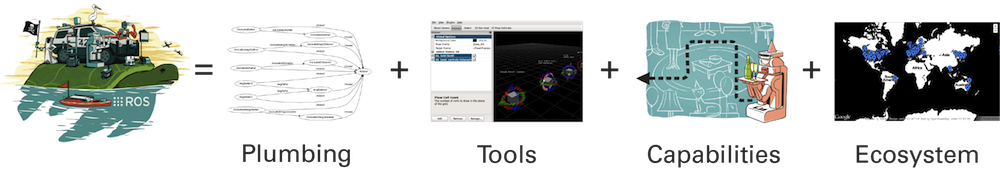
\includegraphics[width=\textwidth]{background/figures/ros_equation.png}
    \caption{\ac{ros} described through a picture, available at the official \ac{ros} website}
    \label{fig:background:ros_equation}
\end{figure}

One also can say that \ac{ros} is a collection of tools, libraries, and conventions that simplify developing a complex robot behavior.
In one interview, Roger Barga, leader of an Amazon's Web Service (AWS RoboMaker), emphasized the importance of \ac{ros} in robotics by saying \textit{``We think that ROS is becoming the Linux for the robots of the future''}\footnote{Roger Barga is an interview by Ricardo Tellez (from The Construct) in ROS Developers podcast -    \url{https://www.theconstructsim.com/aws-robomaker-with-roger-barga/}.}.
Defining \ac{ros} in one sentence is hard, but in further text, two crucial concepts of \ac{ros} will be covered.

The first is the concept of a node.
A task of the node is to perform a computation.
The nodes utilize a publisher-subscriber communication model to exchange messages with each other. 
In that way, the nodes are combined into a graph that can perform more complex tasks.
There are a few important characteristics of each node:
\begin{itemize}
    \item The node can be implemented in various programming languages, without affecting the other nodes.
    Being programming language agnostic allows developers to optimize the nodes for different behaviors.
    For example, if the node has to be efficient or interact closely with the hardware, C programming language may be more suitable.
    Otherwise, if fast prototyping is important,  Python may be a better fit.
    As a result, community nodes are implemented in a programming language that fits best the node's purpose.
    \item The nodes can be run on different computers.
    Each \ac{ros} node includes a mechanism to communicate locally or over the network with the other nodes.
    A complex robotics system often includes multiple powerful computers and dozens of \acp{mcu} or \acp{fpga} specialized for various tasks, and therefore, this ability of \ac{ros} nodes is significant.
    In this project, for example:
    \begin{itemize}
        \item \ac{mcu} is used to execute real-time tasks, like motor control,
        \item on-board computer is used heavy tasks, like perception,
        \item while workstation (\acs{pc}) is used for data visualization, monitoring and debugging.
    \end{itemize}
    \item The nodes can run on virtually any \ac{os}.
    Since \ac{ros2}, Linux, Mac, and Windows are officially supported.
    A stripped version of \ac{ros2}, micro-ROS, runs even on NuttX, FreeRTOS, and Zephyr, and the community has been porting to other \acp{os} as well.
    \item Since \ac{ros2}, the nodes are fully distributed. 
    It means that there is no single message broker to orchestrate the communication.
    Being distributed significantly increases robustness as there is no single point of failure if a node crashes the rest of the system will continue to function.
\end{itemize}

In Fig. \ref{fig:background:ros_nodes} a graph of \ac{ros} nodes is given representing the node concepts given before.

\begin{figure}[H]
    \centering
    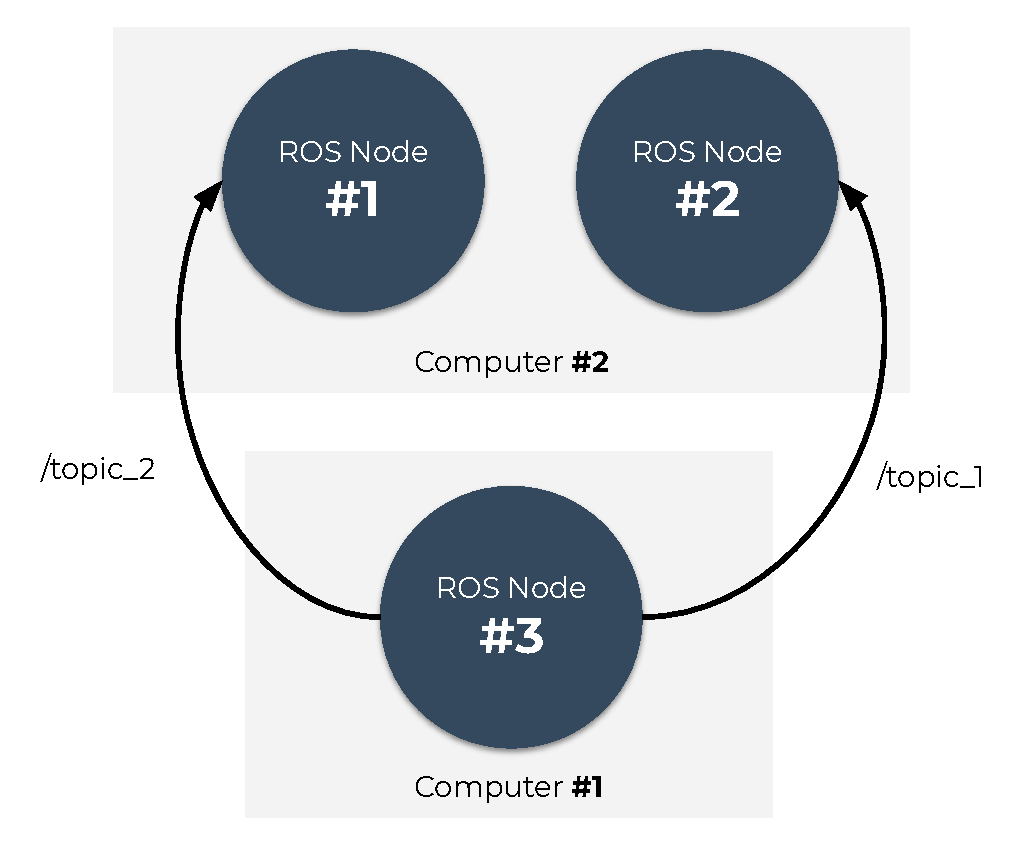
\includegraphics[width=0.8\textwidth]{background/figures/ros_nodes.pdf}
    \caption{General example of three nodes exchange messages through two topics}
    \label{fig:background:ros_nodes}
\end{figure}


The second important concept in \ac{ros} is the means of communication between the nodes.
Mostly, communication between nodes is done through topics, but there other types of communication:
\begin{itemize}
    \item Topics use publisher-subscriber communication model \cite{chen_beaconvey_2018}.
    It means that a node's message will be received by all nodes that are subscribed to the corresponding topic. 
    \ac{qos} was important to \ac{ros} team and therefore, the following \ac{qos} can be defined:
    \begin{itemize}
        \item history, keep last (keep only the last N messages) or keep all,
        \item reliability, best effort (may lose messages if the network is not stable) or reliable (guarantees message delivery) and
        \item durability, transient local (nodes that got subscribed to a topic will receive the last message even though the message is published long time before) or volatile (messages will not be preserved for late-joiners).
    \end{itemize}
    \item Services are used to get a response from the other nodes.
    The concept is very similar to functions with return values.
    A client node sends a service request with data to a node that provides service, and after the result is ready the client node gets the response.
    A typical request can be, \textit{``Is the motor turned on?''} or \textit{``Retrieve the full map now''}.
    \item Parameters allow nodes to be configured by the user or other nodes, on startup or during run-time.
    The underlying implementation is based on the previously explained services.
    I means the nodes can be configured over the network.
    \item Actions are available in \ac{ros} core since \ac{ros2}, and they are similar to the services.
    A difference is that the actions are optimized for requests that generally take longer to execute and need continuous feedback. A typical action can be, \textit{``Move the robot to the new position and while doing it, keep sending me a position''}.
\end{itemize}

The nodes and means of communication between the nodes, are two core concepts of \ac{ros} around which all \ac{ros} tools are built.
Depending on the area of robotics, new concepts may also emerge, but those two are the foundation of the \ac{ros}.

%TODO: \subsection{\ac{ros} Packages}
%TODO: \subsubsection{tf2}
%TODO: \subsection{\ac{ros} Middleware}
%TODO: ROS1 vs ROS2 table


\subsection{\ac{ros} Messages}
One of the sub-objectives of this master project is to provide \ac{ros2} interface that is as compatible as possible with the existing packages.
That will allow users to simply integrate existing \ac{ros2} packages and significantly increase their productivity.
To achieve the objective, \ac{ros2} defines a vast list of existing message, service, and action types.
In the scope of the project, only message types will be further described.

Except for the standard types, available in most programming languages, such as bool, integer, float and string, some messages are more specific to the robotics such as odometry (for describing odometry data), twist (for defining angular and linear velocity), and range (for data from distance sensors).
These messages are exchanged through the previously described topics.
Therefore, integrating a community \ac{ros2} package is a matter of launching (and sometimes configuring it), the package should automatically start publishing and subscribing to the messages as common message types are used.

There are a few groups of message types, some of which are:
\begin{itemize}
    \item \texttt{std\_msgs} is a wrapper around primitive types such as \texttt{Bool}, \texttt{Int32}, \texttt{Float64}, \texttt{String} and \texttt{Float64MultiArray}.
    These message types are usually used to compose more complex message types and in general should be avoidable if there is more suitable type from the other groups.
    \item \texttt{geometry\_msgs} contains geometry primitives.
    For example \texttt{Twist} is used to describe linear and angular velocity (usually used to control robot's velocity), rotations are described with \texttt{Quaternion} message types, robot's pose \texttt{Pose} (e.g. the navigation stack uses this message type describe the robot's goal position and orientation) and \texttt{Transform} to describe relative orientation and translation of two frames.
    \item \texttt{nav\_msgs} group contains message types used to interact with the navigation stack and the related packages.
    It defines message types such as \texttt{OccupancyGrid} that represent a map and \texttt{Odometry} that contains odometry data. 
    \item \texttt{sensor\_msgs} contains message types that are commonly used to describe data from sensor such as distance sensors (\texttt{Range}), \acsp{lidar} (\texttt{LaserScan}), cameras (\texttt{CameraInfo} and \texttt{Image}), light sensors (\texttt{Illuminance}) and similar. 
\end{itemize}

There are many more message group types, but those are the most relevant ones for this project.

\subsection{\ac{ros} Distributions}

\ac{ros} distributions is another vital aspect of the project.
The newest \ac{ros} distribution (as of the time of writing the thesis) is deliberately chosen.
The choice is will be described later, but first, \ac{ros} versioning has to be described.

\ac{ros} team releases a new \ac{ros} distribution every six months, following Ubuntu's release cycle.
Every two years a new \ac{ros} \ac{lts} is released,
a few weeks after Ubuntu's \ac{lts} release, as \ac{ros} relies on the latest Ubuntu \ac{lts}.

In December 2017, \ac{ros2} is introduced, and since then \ac{ros} team has been publishing \ac{ros} and \ac{ros} releases every six months.
\ac{ros2} should fully replace the \ac{ros1} once \ac{ros2} mature\footnote{Dirk Thomas, principle software engineer working on \ac{ros} core, wrote about \ac{ros} future at \ac{ros} Discourse -  \url{https://discourse.ros.org/t/planning-future-ros-1-distribution-s/6538}. He stated \ac{ros1} will be most probably supported until 2025 and then it should be completely replaced by \ac{ros2}}.

\begin{figure}[H]
    \centering
    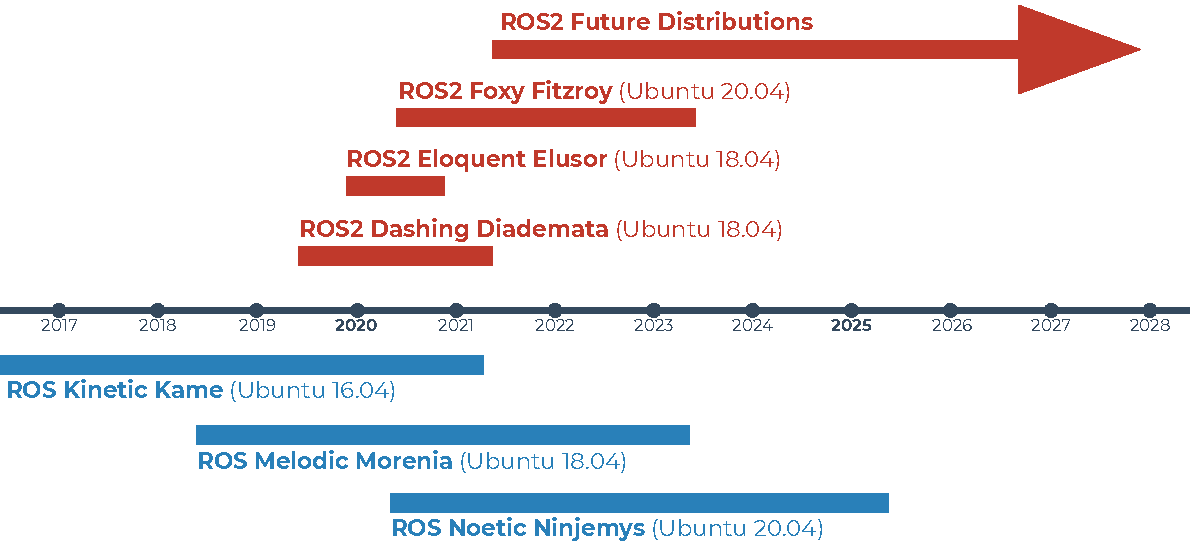
\includegraphics[width=\textwidth]{background/figures/ros_distributions}
    \caption{Timeline of \ac{ros1} and \ac{ros2} distributions}
    \label{fig:background:ros_distributions}
\end{figure}

In Fig. \ref{fig:background:ros_distributions} a few latest \ac{ros} distributions are shown.
Note that they all rely on Ubuntu \ac{lts} distributions and that \ac{ros2} Foxy Fitzroy is the first \ac{ros2} distribution with three years of support.

In this project, the importance of \ac{ros2} is recognized, and therefore it is chosen instead of \ac{ros1}.
Also, the master project had started before \ac{ros2} Foxy Fitzroy was released, and therefore the initial code is written for \ac{ros2} Eloquent Elusor with a plan to adopt \ac{ros2} Foxy Fitzroy.
Finally, the master project is compatible with \ac{ros2} Eloquent Elusor and \ac{ros2} Foxy Fitzroy.

\section{Robotics Platforms}
The project's main objective is to introduce \ac{ros2} support for the e-puck2 physical and simulated robot, and other simulated robots while focusing on Khepera IV.
Therefore, those two robots are will be described in more detail.

\subsection{E-puck2}
E-puck2 is the second generation of the e-puck robot\cite{mondada_e-puck_nodate}.
E-pucks are small differential wheeled robots (e-puck and e-puck2 have the same footprint) with a radius of 35mm.
As a miniature robot, it is the perfect candidate for education and multi-robot research.
It is originally designed for micro-engineering education by Michael Bonani and Francesco Mondada at \ac{epfl}.
The robot is open hardware, and the software is open-source.

\begin{figure}[H]
    \centering
    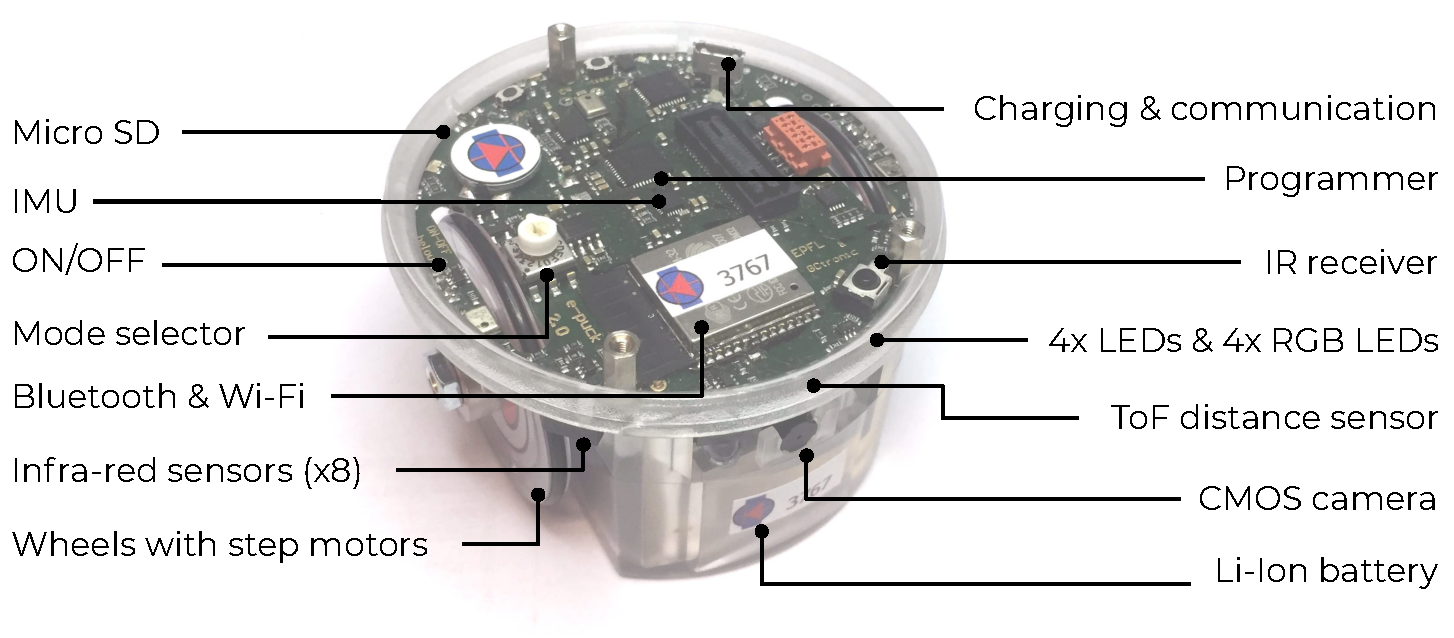
\includegraphics[width=\textwidth]{background/figures/epuck2.pdf}
    \caption{E-puck2 robot with list of main components}
    \label{fig:background:e-puck2}
\end{figure}

The robot is shown in Fig. \ref{fig:background:e-puck2} and its main specifications are given in Table. \ref{tab:background:specifications}.

\begin{table}[H]
    \begin{adjustwidth}{-1.5in}{-1.5in}
    \centering
    \begin{tabular}{|l|l|}
        \hline
        Size, weight & 70mm diameter, 130g \\
        \hline
        \ac{mcu} & 32-bit STM32F407 @ 168 MHz (210 \acs{mips}), \acs{dsp} and \acs{fpu}, \acs{dma} \\
        \hline
        Motors & 2 stepper motors, 50:1 reduction gear and 20 steps per revolution \\
        \hline
        Max velocity & 0.154m/s \\
        \hline
        Distance sensor & 8 infra-red sensors (up to 0.06m) and one \acs{tof} (up to 2m) \\
        \hline
        Camera & 640x480 at 15\acs{fps} \\
        \hline
        \acs{imu} & 3D accelerometer, 3D gyro, 3D magnetometer \\
        \hline
        \acsp{led} & 4 red \acsp{led} and 4 \acs{rgb} \acsp{led} \\
        \hline
    \end{tabular}
    \end{adjustwidth}
    \caption{Relevant specifications of e-puck2 robot}
    \label{tab:background:specifications}
\end{table}

\subsubsection{Pi-puck}

E-puck2 robot allows extensions to be added providing different features such as additional autonomy, ground sensors or additional processing power.
The pi-puck extension, for example, consists of a Raspberry Pi Zero W and adapter \ac{pcb}, and interacts directly with on-board \ac{mcu} and sensors \cite{millard_pi-puck_2017}.
Since Raspberry Pi Zero W is Linux base board it can run \ac{ros} with full \ac{dds} implementation.

\begin{figure}[H]
    \centering
    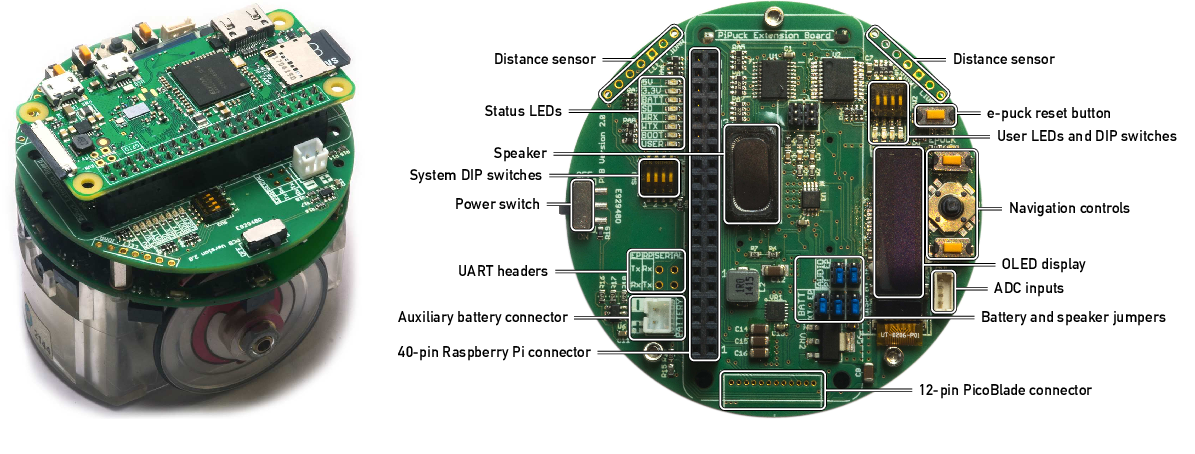
\includegraphics[width=\textwidth]{background/figures/pi-puck.png}
    \caption{Pi-puck extension consist of two parts, \ac{pcb} and Raspberry Pi Zero W \cite{millard_pi-puck_2017}}
    \label{fig:background:pi-puck}
\end{figure}

In the project, Raspberry Pi Zero W allows us to run \ac{ros2} nodes on the robot and execute complex operations such as \acs{jpeg} image compression that otherwise would not be possible.

\subsection{Khepera IV}

Khepera IV is a similar robot to e-puck2, but is more prominent in size (with a radius of 70mm), and has more powerful sensors and computational units \cite{reis_khepera_2016}.
The robot is designed by K-Team\footnote{Official website of K-Team is available at \url{https://www.k-team.com/}.} to fit any indoor lab application.

\begin{figure}[H]
    \centering
    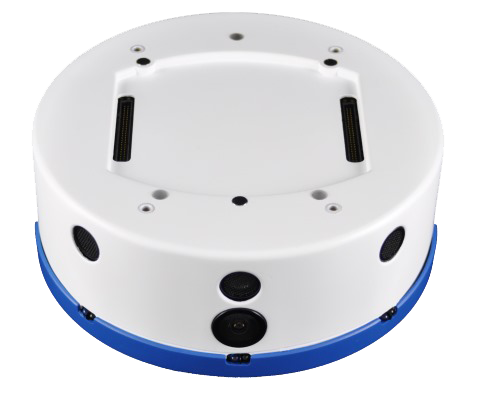
\includegraphics[width=0.6\textwidth]{background/figures/khepera_iv.png}
    \caption{Khepera IV robot \cite{reis_khepera_2016}}
    \label{fig:background:khepera_iv}
\end{figure}

The robot is shown in Fig. \ref{fig:background:khepera_iv} and its main specifications are given in Table. \ref{tab:background:khepera_iv}.

\begin{table}[H]
    \centering
    \begin{tabular}{|l|l|}
        \hline
        Size, weight & 140mm diameter, 540g \\
        \hline
        Processor & 800MHz ARM Cortex-A8 Processor and \acs{mcu} \\
        \hline
        Motors & 2 DC brushed motors with incremental encoders \\
        \hline
        Max velocity & 0.8m/s \\
        \hline
        Distance sensor & 8 infra-red (up to 0.25m) and 5 ultrasonic (up to 2m) \\
        \hline
        Camera & 752x480 at 30\acs{fps} \\
        \hline
        \acs{imu} & 3D accelerometer, 3D gyro \\
        \hline
        \acsp{led} & 3 \acs{rgb} \acsp{led} \\
        \hline
    \end{tabular}
    \caption{Relevant specifications of Khepera IV robot}
    \label{tab:background:khepera_iv}
\end{table}

\section{Webots}
Webots is an open-source robot simulator developed by Cyberbotics\footnote{Official website of Cyberbotics is available at \url{https://cyberbotics.com/}.}, initially designed at \ac{epfl}.
The simulator provides a development environment to model, program and simulate robots \cite{michel_cyberbotics_2004, michel_webots_1998, michel_cyberbotics_2014}.

\begin{figure}[H]
    \centering
    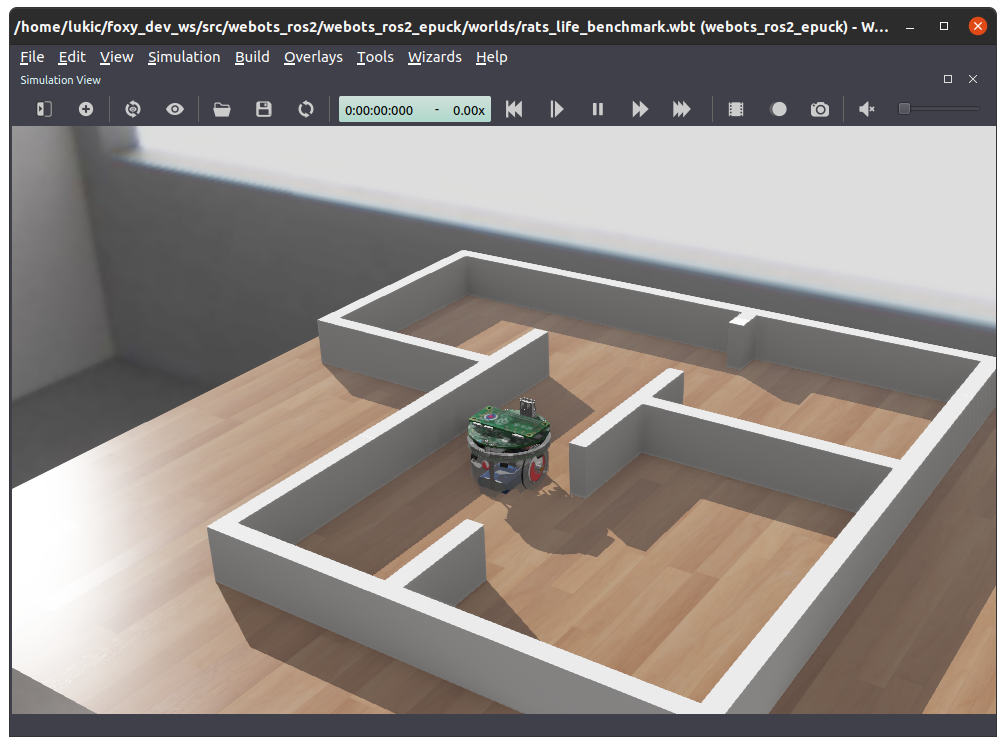
\includegraphics[width=\textwidth]{background/figures/webots.png}
    \caption{Webots robot simulator: e-puck2 robot on a table}
    \label{fig:background:webots}
\end{figure}

The main Webots features are:
\begin{itemize}
    \item Robot/world editor: The models are stored in VRML97 format, allowing users to either change the document manually or through the Webots user interface. 
    The Webots world editor allows the users to see changes in the world immediately.
    It is possible to include pre-built models, and the users can choose among a huge library of models.
    \item Realistic simulation: The simulations produced in Webots are realistic compared to the similar products. 
    The physics simulation is based on a modified version of \ac{ode}.
    The models shipped with the Webots are visually very detailed, although still optimized for high performance.
    \item Programming interface: \ac{api} for programming robots is officially available in the most popular programming languages, C, C++, Python, MATLAB and Java, while community-contributed packages further extend this list\footnote{An example of \ac{api} in Haskell programming language, created by the community, is available at \url{https://github.com/cyberbotics/HsWebots}.}.
    The \ac{api} allows simple access to the sensors and actuators available in the robots.
    \item Deterministic simulations: Webots guarantees a simulation to output the same behavior every time it runs (user can also choose non-deterministic simulation).
    Although a non-deterministic simulation is preferable before transferring to a real robot, deterministic simulation is beneficial when doing initial algorithm tests.
    Also, this feature can be exploited to simplify automated testing in \ac{ci}.
\end{itemize}

Those are the main points that justify the usage of Webots over similar products.

\section{Related Work}
Existing \ac{ros} support for the e-puck2 physical robot and Webots will be analyzed.
Drawbacks in current implementations of \ac{ros} support are the motivation for this project; therefore, they will be explained in this section.

\subsection{\ac{ros} Support for E-puck2}
GCtronic, a company behind e-puck robots, has two types of \ac{ros} drivers available.
The first is made for e-puck robots without pi-puck extension\footnote{\ac{ros} driver that doesn't run on pi-puck extension is available at \url{https://github.com/gctronic/epuck_driver_cpp/tree/e-puck2}.}.
In that case, \ac{ros} driver runs on a workstation while communicating with the e-puck over Bluetooth. The second \ac{ros} driver implementation runs on pi-puck extension\footnote{\ac{ros} driver that uses pi-puck extension is available at \url{https://github.com/gctronic/epuck_driver_cpp/tree/pi-puck}.} and it is similar to the \ac{ros} driver we aim to develop. The main drawbacks are that it is not available for \ac{ros2}, it is not unit tested nor code quality tested, it does not include a camera driver, and there is no comprehensive documentation.

\begin{table}[H]
    \begin{adjustwidth}{-1.5in}{-1.5in}
    \centering
    \begin{tabular}{|l|c|c|c|}
         \hline
         & \textbf{GCtronic's \#1} & \textbf{GCtronic's \#2} & \textbf{Proposed solution} \\
         \hline
         \rowcolor{lightgray} \textbf{\ac{ros2} support} & No & No & Yes \\
         \hline
         \rowcolor{lightgray} \textbf{Communication} & Bluetooth & \acs{udpros}/\acs{tcpros} & \ac{dds} \\
         \hline
         \rowcolor{lightgray} \textbf{Camera} & 160x120@4 & No & 640x480@10 \\
         \hline
         \textbf{Battery autonomy} & Long & Short & Short \\
         \hline
         \rowcolor{lightgray} \textbf{Unit tests} & No & No & Yes, with \ac{ci} \\
         \hline
         \rowcolor{lightgray} \textbf{Code quality tests} & No & No & Yes, with \ac{ci} \\
         \hline
         \rowcolor{lightgray} \textbf{Cross-compilation} & No & No & Yes, tools are given  \\
         \hline
         \rowcolor{lightgray} \textbf{Independent from \acs{pc}} & No & Yes & Yes  \\
         \hline
    \end{tabular}
    \end{adjustwidth}
    \caption[Comparison of the proposed \ac{ros} drive with the existing implementations]{Comparison of the proposed \ac{ros2} driver with the existing implementations (aspects in which the proposed solution is better are highlighted).}
    \label{tab:background:epuck_ros}
\end{table}

As showed in Table \ref{tab:background:epuck_ros} the proposed solution offers better implementation in many aspects.
The proposed solution's main drawback is the battery autonomy as the pi-puck extension requires a significant amount of power (around 0.7 watts, it can vary depending on usage).


\subsection{\ac{ros} Support in Webots}
A major part of the master project is the improvement of \ac{ros2} support for Webots.
Webots supports both, \ac{ros1} and \ac{ros2}, but with certain limitations.

Webots \ac{ros1} implementation automatically exposes all Webots \ac{api} functions as \ac{ros} topics and services.
Automatically exposing \ac{ros} \ac{api} sounds as a reasonable solution, but it is uncanny for the \ac{ros} ecosystem, and therefore, much effort is required from users to adapt the exposed \ac{api} to fit other \ac{ros} packages.
For example, if one wants to publish odometry data, the one needs to create a \ac{ros} node that subscribes topics published by encoders and then publishes the corresponding odometry and transform messages. This work is time consuming, complex, and consumes unnecessary processing power by republishing all the messages.

Therefore, Cyberbotics has taken another approach in \ac{ros2} support.
Instead of creating \ac{ros2} topics and services as done for \ac{ros1} it provides facilities to users to design and implement their own \ac{ros2} interface using Webots \ac{api} functions.
Creating a specific \ac{ros2} driver simplifies usage, but it is still time-consuming as the \ac{ros2} driver has to be created for each robot.

This project extends Webots' support for \ac{ros2} by adding modules that can automatically create \ac{ros2} interface, compatible with other \ac{ros2} packages, based on a robot description.
For the previously mentioned example, in which odometry has to be published, the proposed improvement will allow automatic publishing of odometry and transform messages, including support for \ac{ros2} parameters and velocity control of the robots.

This improvement should allow users to integrate Webots simulations faster in their \ac{ros2} applications, and it should effectively lead to a greater adoption of robot simulations among the \ac{ros2} community that uses Webots.
